\documentclass[fleqn,usenatbib]{mnras}

\usepackage{newtxtext,newtxmath}
\usepackage[T1]{fontenc}
\DeclareRobustCommand{\VAN}[3]{#2}
\let\VANthebibliography\thebibliography
\def\thebibliography{\DeclareRobustCommand{\VAN}[3]{##3}\VANthebibliography}
\usepackage{graphicx}	% Including figure files
\usepackage{amsmath}	% Advanced maths commands
%\usepackage{amssymb}	% Extra maths symbols

%%%%%%%%%%%%%%%%%%%%%%%%%%%%%%%%%%%%%%%%%%%%%%%%%%

%%%%% AUTHORS - PLACE YOUR OWN COMMANDS HERE %%%%%

% Please keep new commands to a minimum, and use \newcommand not \def to avoid
% overwriting existing commands. Example:
%\newcommand{\pcm}{\,cm$^{-2}$}	% per cm-squared

%%%%%%%%%%%%%%%%%%%%%%%%%%%%%%%%%%%%%%%%%%%%%%%%%%

%%%%%%%%%%%%%%%%%%% TITLE PAGE %%%%%%%%%%%%%%%%%%%

% Title of the paper, and the short title which is used in the headers.
% Keep the title short and informative.
\title[Artificial Pulsar]{Tuning Low Frequency Pulsar Searching with an  Artificial Pulsar Device}

\author[J.-H. Gu et al.]{
Junhua Gu$^{1}$\thanks{E-mail: jhgu@nao.cas.cn} et al.
\\
% List of institutions
$^{1}$National Astronomical Observatories, Chinese Academy of Sciences, 20A Datun Road, Beijing, China
}
% These dates will be filled out by the publisher
\date{Accepted XXX. Received YYY; in original form ZZZ}

% Enter the current year, for the copyright statements etc.
\pubyear{2021}

% Don't change these lines
\begin{document}
\label{firstpage}
\pagerange{\pageref{firstpage}--\pageref{lastpage}}
\maketitle

% Abstract of the paper
\begin{abstract}
Abstract
\end{abstract}

% Select between one and six entries from the list of approved keywords.
% Don't make up new ones.
\begin{keywords}
keyword1 -- keyword2 -- keyword3
\end{keywords}

\section{Introduction}
\citet{2017AAS...22915516P}, \citet{2011AAS...21723406S}

\section{Artificial Pulsar Device}
The artificial pulsar device (APD hereafter) is a device that is able to emit simulated pulsar signal within some certain bandpass.
We design it to be able to simulate the dispersion effect and arbitrary pulse profile of a pulsar.
Our implementation of APD is composed of three modules: 1) a high performance workstation that is responsible of computing the pulsar signal online, 2) a software-defined radio transmitter that receives the command from the workstation and convert it to voltage signal, which is then fed into 3) a radio frequency front-end. 
The radio frequency front-end is further composed of a radio frequency power amplifier (RFPA hereafter) and an antenna that is used to broadcast the actual signal.

\begin{figure}
    \centering
    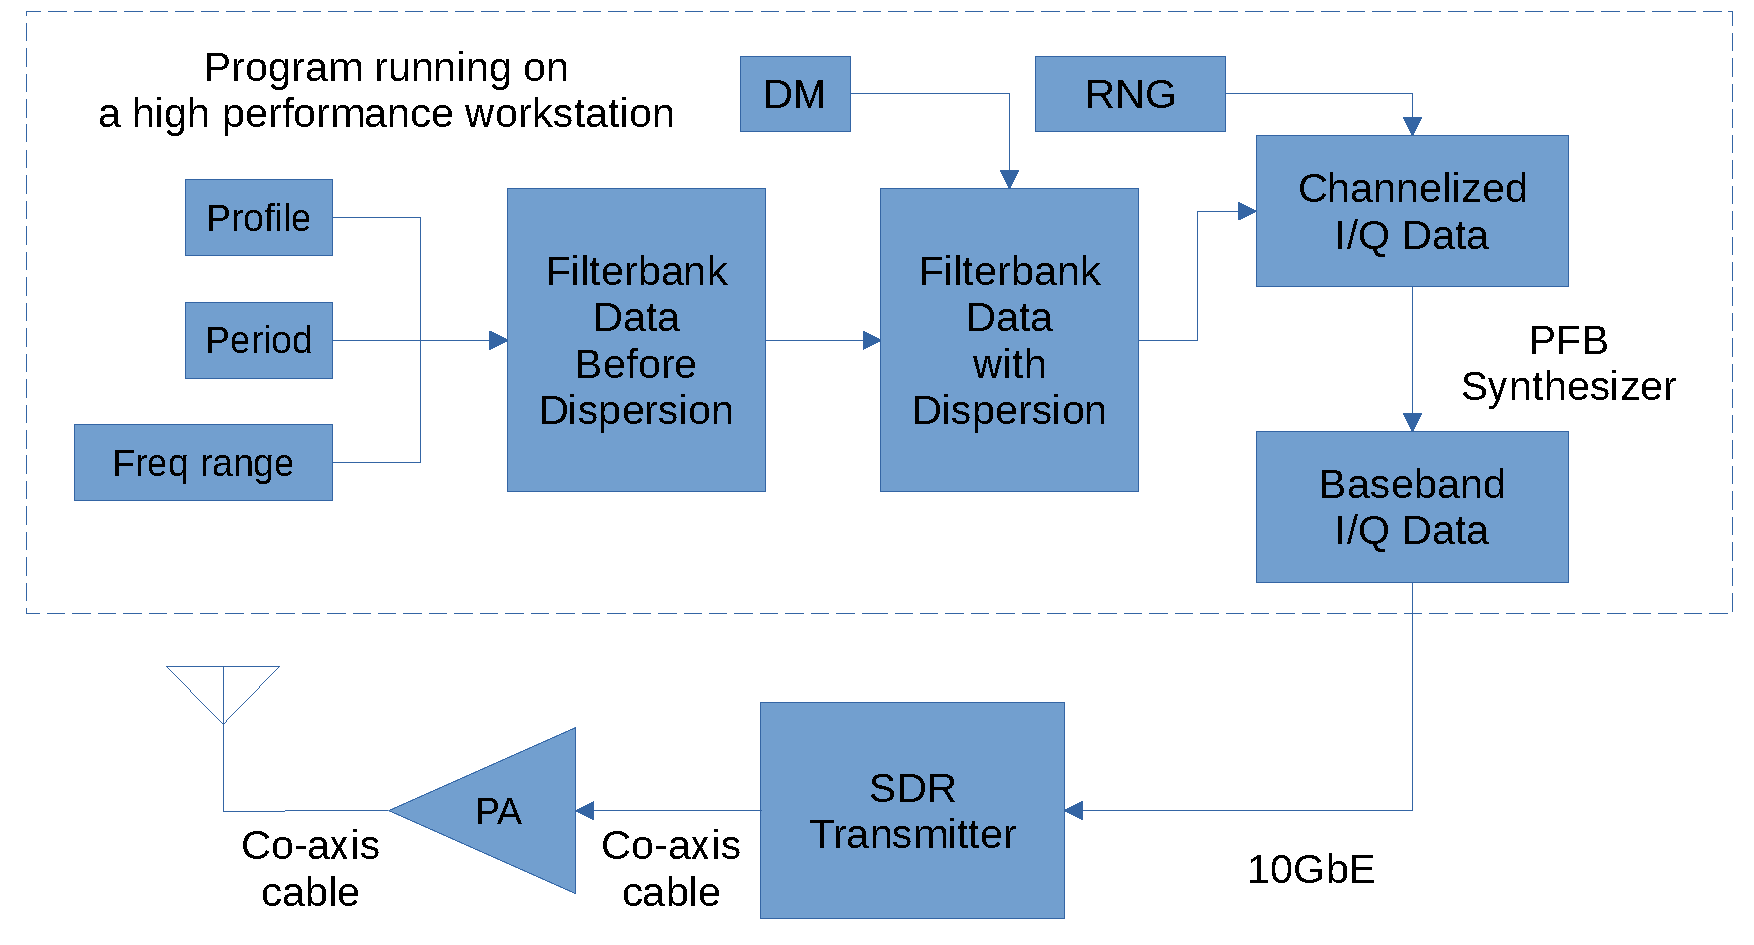
\includegraphics[width=0.95\columnwidth]{flow_chart.pdf}
    \caption{The flow chart of emitting the simulated pulsar signal.
    }
    \label{fig:flow_chart}
\end{figure}


The APD can be placed near the low-frequency pulsar observation device (LFPOD hereafter). 
It is not necessary for the emitting antenna to be placed inside the range of the primary beam LFPOD.
The power of the emitted signal can be amplified to a high enough level so that when the signal is received by the LFPOD from its side lobes it approximates the power level of a natural pulsar.

\subsection{Computing Artificial Pulsar Signal}

\subsection{Emitting Generated Signal}

\section{An Example of Tuning}

\section{Discussion}

\section{Conclusions}

\section*{Acknowledgements}


%%%%%%%%%%%%%%%%%%%%%%%%%%%%%%%%%%%%%%%%%%%%%%%%%%

\bibliographystyle{mnras}
\bibliography{ms}

%%%%%%%%%%%%%%%%%%%%%%%%%%%%%%%%%%%%%%%%%%%%%%%%%%


% Don't change these lines
\bsp	% typesetting comment
\label{lastpage}
\end{document}

% End of ms.tex
